\documentclass[]{article}

%%%%%%%%%%%%%%%%%%%%%%%%%%%%%%%%%%%%%%%%%%%%%%%%%%%%%%%%%%%%%%%%%%%%%%%
% Definicion de paquetes
\usepackage{minted}
\usepackage[utf8]{inputenc}
\usepackage[spanish]{babel}
\usepackage{xcolor}
\usepackage{graphicx}

%%%%%%%%%%%%%%%%%%%%%%%%%%%%%%%%%%%%%%%%%%%%%%%%%%%%%%%%%%%%%%%%%%%%%%%
% Definición de comandos
\definecolor{LightGray}{gray}{0.85}
\renewcommand\listingscaption{Listado}
\graphicspath{ {./images/} }

%%%%%%%%%%%%%%%%%%%%%%%%%%%%%%%%%%%%%%%%%%%%%%%%%%%%%%%%%%%%%%%%%%%%%%%
%% Empieza el documento
\begin{document}
  \title{Práctica 1}
  \author{Miguel Emilio Ruiz Nieto}
  \maketitle

  \section*{Ejercicio 2}

  Ejecución de la clase Agente:

  \begin{minted}{bash}
    $ java -classpath ./lib/jade.jar:./src jade.Boot -gui Bob:Agente
    $ java -classpath ./lib/jade.jar:./src jade.Boot -gui Mary:Agente
    $ java -classpath ./lib/jade.jar:./src jade.Boot -gui Peter:Agente
  \end{minted}

  A continuación se muestran las respectivas salidas de cada ejecución,
  junto a lo que se muestra dentro de la interfaz gráfica:

  \begin{listing}
  \begin{minted}
    [
      baselinestretch=1.2,
      bgcolor=LightGray,
      fontsize=\small
    ]{text}
    $ java -classpath ./lib/jade.jar:./src jade.Boot -gui Bob:Agente

    Feb 27, 2022 12:18:30 PM jade.core.Runtime beginContainer
    INFO: ----------------------------------
        This is JADE 4.5.0 - revision 6825 of 23-05-2017 10:06:04
        downloaded in Open Source, under LGPL restrictions,
        at http://jade.tilab.com/
    ----------------------------------------
    Feb 27, 2022 12:18:30 PM jade.imtp.leap.LEAPIMTPManager initialize
    INFO: Listening for intra-platform commands on address:
    - jicp://172.17.0.1:1099

    Feb 27, 2022 12:18:31 PM jade.core.BaseService init
    INFO: Service jade.core.management.AgentManagement initialized
    Feb 27, 2022 12:18:31 PM jade.core.BaseService init
    INFO: Service jade.core.messaging.Messaging initialized
    Feb 27, 2022 12:18:31 PM jade.core.BaseService init
    INFO: Service jade.core.resource.ResourceManagement initialized
    Feb 27, 2022 12:18:31 PM jade.core.BaseService init
    INFO: Service jade.core.mobility.AgentMobility initialized
    Feb 27, 2022 12:18:31 PM jade.core.BaseService init
    INFO: Service jade.core.event.Notification initialized
    Feb 27, 2022 12:18:31 PM jade.mtp.http.HTTPServer <init>
    INFO: HTTP-MTP Using XML parser
    com.sun.org.apache.xerces.internal.jaxp.SAXParserImpl$JAXPSAXParser
    Feb 27, 2022 12:18:31 PM jade.core.messaging.MessagingService boot
    INFO: MTP addresses:
    http://precision-5520:7778/acc
    Feb 27, 2022 12:18:31 PM jade.core.AgentContainerImpl joinPlatform
    INFO: --------------------------------------
    Agent container Main-Container@172.17.0.1 is ready.
    --------------------------------------------
    Hola! Soy el AgenteMinimo Bob@172.17.0.1:1099/JADE
  \end{minted}
  \caption{Primera ejecución}
  \end{listing}

  \begin{listing}
  \begin{minted}
    [
      baselinestretch=1.2,
      bgcolor=LightGray,
      fontsize=\small
    ]{text}
    $ java -classpath ./lib/jade.jar:./src jade.Boot -gui Mary:Agente

    Feb 27, 2022 12:33:30 PM jade.core.Runtime beginContainer
    INFO: ----------------------------------
        This is JADE 4.5.0 - revision 6825 of 23-05-2017 10:06:04
        downloaded in Open Source, under LGPL restrictions,
        at http://jade.tilab.com/
    ----------------------------------------
    Feb 27, 2022 12:33:30 PM jade.imtp.leap.LEAPIMTPManager initialize
    INFO: Listening for intra-platform commands on address:
    - jicp://172.17.0.1:1099

    Feb 27, 2022 12:33:31 PM jade.core.BaseService init
    INFO: Service jade.core.management.AgentManagement initialized
    Feb 27, 2022 12:33:31 PM jade.core.BaseService init
    INFO: Service jade.core.messaging.Messaging initialized
    Feb 27, 2022 12:33:31 PM jade.core.BaseService init
    INFO: Service jade.core.resource.ResourceManagement initialized
    Feb 27, 2022 12:33:31 PM jade.core.BaseService init
    INFO: Service jade.core.mobility.AgentMobility initialized
    Feb 27, 2022 12:33:31 PM jade.core.BaseService init
    INFO: Service jade.core.event.Notification initialized
    Feb 27, 2022 12:33:31 PM jade.mtp.http.HTTPServer <init>
    INFO: HTTP-MTP Using XML parser
    com.sun.org.apache.xerces.internal.jaxp.SAXParserImpl$JAXPSAXParser
    Feb 27, 2022 12:33:31 PM jade.core.messaging.MessagingService boot
    INFO: MTP addresses:
    http://precision-5520:7778/acc
    Hola! Soy el AgenteMinimo Mary@172.17.0.1:1099/JADE
    Feb 27, 2022 12:33:31 PM jade.core.AgentContainerImpl joinPlatform
    INFO: --------------------------------------
    Agent container Main-Container@172.17.0.1 is ready.
  \end{minted}
  \caption{Segunda ejecución}
  \end{listing}

  \begin{listing}
  \begin{minted}
    [
      baselinestretch=1.2,
      bgcolor=LightGray,
      fontsize=\small
    ]{text}
    $ java -classpath ./lib/jade.jar:./src jade.Boot -gui Peter:Agente

    Feb 27, 2022 12:35:40 PM jade.core.Runtime beginContainer
    INFO: ----------------------------------
        This is JADE 4.5.0 - revision 6825 of 23-05-2017 10:06:04
        downloaded in Open Source, under LGPL restrictions,
        at http://jade.tilab.com/
    ----------------------------------------
    Feb 27, 2022 12:35:40 PM jade.imtp.leap.LEAPIMTPManager initialize
    INFO: Listening for intra-platform commands on address:
    - jicp://172.17.0.1:1099

    Feb 27, 2022 12:35:41 PM jade.core.BaseService init
    INFO: Service jade.core.management.AgentManagement initialized
    Feb 27, 2022 12:35:41 PM jade.core.BaseService init
    INFO: Service jade.core.messaging.Messaging initialized
    Feb 27, 2022 12:35:41 PM jade.core.BaseService init
    INFO: Service jade.core.resource.ResourceManagement initialized
    Feb 27, 2022 12:35:41 PM jade.core.BaseService init
    INFO: Service jade.core.mobility.AgentMobility initialized
    Feb 27, 2022 12:35:41 PM jade.core.BaseService init
    INFO: Service jade.core.event.Notification initialized
    Feb 27, 2022 12:35:41 PM jade.mtp.http.HTTPServer <init>
    INFO: HTTP-MTP Using XML parser
    com.sun.org.apache.xerces.internal.jaxp.SAXParserImpl$JAXPSAXParser
    Feb 27, 2022 12:35:41 PM jade.core.messaging.MessagingService boot
    INFO: MTP addresses:
    http://precision-5520:7778/acc
    Hola! Soy el AgenteMinimo Peter@172.17.0.1:1099/JADE
    Feb 27, 2022 12:35:41 PM jade.core.AgentContainerImpl joinPlatform
    INFO: --------------------------------------
    Agent container Main-Container@172.17.0.1 is ready.
    --------------------------------------------
  \end{minted}
  \caption{Tercera ejecución}
  \end{listing}

  \newpage

  \begin{figure}[h]
    \centering
    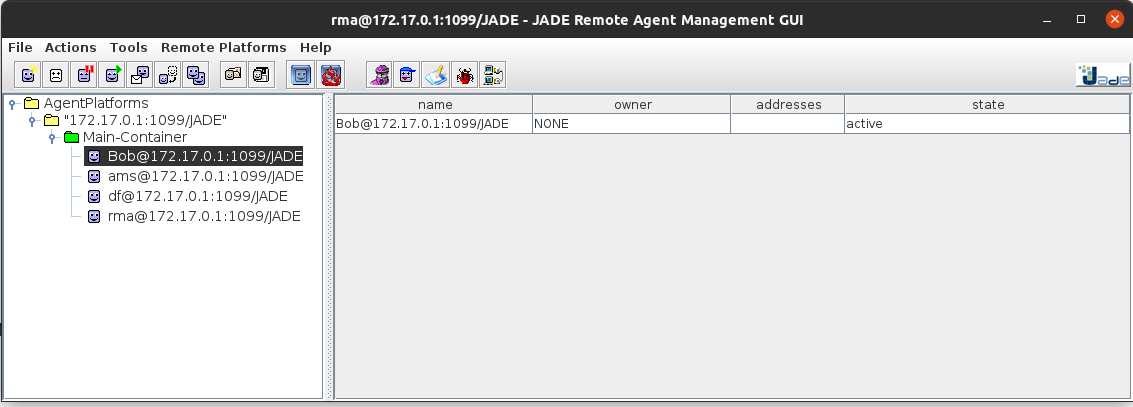
\includegraphics[width=\textwidth]{bob.png}
    \caption{Agente Bob}
  \end{figure}

  \begin{figure}[h]
    \centering
    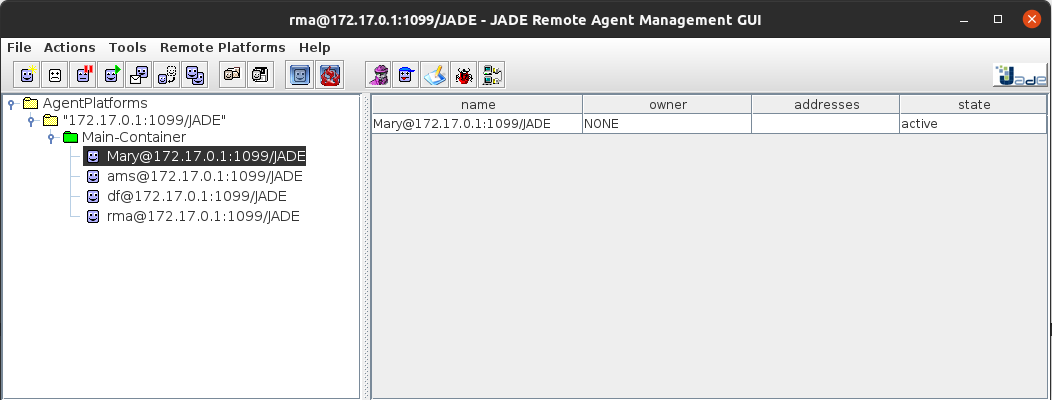
\includegraphics[width=\textwidth]{mary.png}
    \caption{Agente Mary}
  \end{figure}

  \begin{figure}[h]
    \centering
    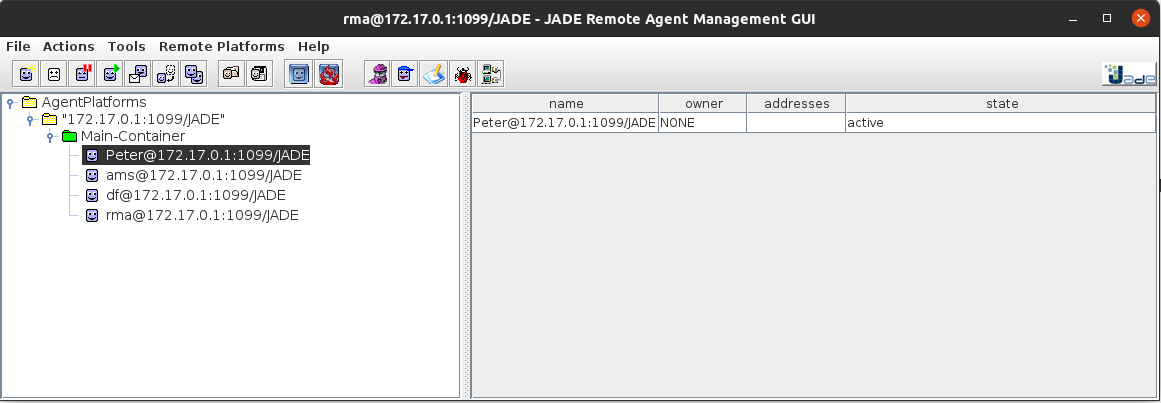
\includegraphics[width=\textwidth]{peter.png}
    \caption{Agente Peter}
  \end{figure}

  \newpage

  Podemos observar de las distintas ejecuciones que el agente toma el nombre
  que le hemos pasado como argumento dentro del mensaje:

  \mint{text}|Hola! Soy el AgenteMinimo Peter@172.17.0.1:1099/JADE|

  % TODO añadir capturas de cada salida
\end{document}